\documentclass{beamer}

%
% Choose how your presentation looks.
%
% For more themes, color themes and font themes, see:
% http://deic.uab.es/~iblanes/beamer_gallery/index_by_theme.html
%
\mode<presentation>
{
  \usetheme{default}      % or try Darmstadt, Madrid, Warsaw, ...
  \usecolortheme{default} % or try albatross, beaver, crane, ...
  \usefonttheme{default}  % or try serif, structurebold, ...
  \setbeamertemplate{navigation symbols}{}
  \setbeamertemplate{caption}[numbered]
  \setbeamertemplate{footline}[page number]
  \setbeamercolor{frametitle}{fg=white}
  \setbeamercolor{footline}{fg=black}
} 

\usepackage[english]{babel}
\usepackage[utf8x]{inputenc}
\usepackage{tikz}
\usepackage{listings}
\usepackage{courier}

\xdefinecolor{darkblue}{rgb}{0.1,0.1,0.7}
\xdefinecolor{dianablue}{rgb}{0.18,0.24,0.31}
\definecolor{commentgreen}{rgb}{0,0.6,0}
\definecolor{stringmauve}{rgb}{0.58,0,0.82}

\lstset{ %
  backgroundcolor=\color{white},      % choose the background color
  basicstyle=\ttfamily\small,         % size of fonts used for the code
  breaklines=true,                    % automatic line breaking only at whitespace
  captionpos=b,                       % sets the caption-position to bottom
  commentstyle=\color{commentgreen},  % comment style
  escapeinside={\%*}{*)},             % if you want to add LaTeX within your code
  keywordstyle=\color{blue},          % keyword style
  stringstyle=\color{stringmauve},    % string literal style
  showstringspaces=false,
  showlines=true
}

\lstdefinelanguage{scala}{
  morekeywords={abstract,case,catch,class,def,%
    do,else,extends,false,final,finally,%
    for,if,implicit,import,match,mixin,%
    new,null,object,override,package,%
    private,protected,requires,return,sealed,%
    super,this,throw,trait,true,try,%
    type,val,var,while,with,yield},
  otherkeywords={=>,<-,<\%,<:,>:,\#,@},
  sensitive=true,
  morecomment=[l]{//},
  morecomment=[n]{/*}{*/},
  morestring=[b]",
  morestring=[b]',
  morestring=[b]"""
}

\title[2016-09-30-gpudb]{GPU-enabled physics event database}
\author{Jim Pivarski}
\institute{Princeton -- DIANA}
\date{September 30, 2016}

\begin{document}

\logo{\pgfputat{\pgfxy(0.11, 8)}{\pgfbox[right,base]{\tikz{\filldraw[fill=dianablue, draw=none] (0 cm, 0 cm) rectangle (50 cm, 1 cm);}}}\pgfputat{\pgfxy(0.11, -0.6)}{\pgfbox[right,base]{\tikz{\filldraw[fill=dianablue, draw=none] (0 cm, 0 cm) rectangle (50 cm, 1 cm);}\includegraphics[height=0.99 cm]{diana-hep-logo.png}\tikz{\filldraw[fill=dianablue, draw=none] (0 cm, 0 cm) rectangle (4.9 cm, 1 cm);}}}}

\begin{frame}
  \titlepage
\end{frame}

\logo{\pgfputat{\pgfxy(0.11, 8)}{\pgfbox[right,base]{\tikz{\filldraw[fill=dianablue, draw=none] (0 cm, 0 cm) rectangle (50 cm, 1 cm);}\includegraphics[height=1 cm]{diana-hep-logo.png}}}}

% Uncomment these lines for an automatically generated outline.
%\begin{frame}{Outline}
%  \tableofcontents
%\end{frame}

\begin{frame}{Current physics workflow}
\vspace{0.5 cm}
\only<1>{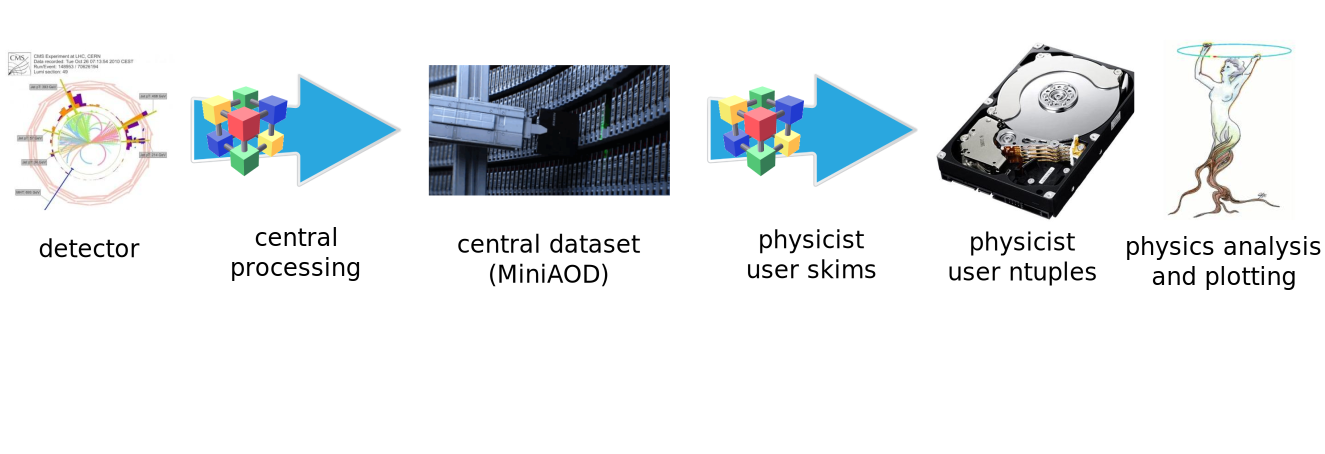
\includegraphics[width=\linewidth]{workflow1.pdf}}
\only<2->{\includegraphics[width=\linewidth]{workflow2.pdf}}

\vspace{0.25 cm}
\begin{itemize}
\item<3-> Event index database addresses one part of the slowness of physicist user skims at a cost of adding a layer of complexity.
\item<4-> I am now discovering that there are much worse hotspots in the physicists' scripts.
\item<5-> Bugs, inefficiencies in the custom code and ntuple-version control issues get in the way of physicists doing analysis.
\end{itemize}
\end{frame}

\begin{frame}{Ideal physics workflow}
\vspace{0.5 cm}
\includegraphics[width=\linewidth]{workflow3.pdf}

\vspace{0.25 cm}
\begin{itemize}
\item Ideally, data should go directly from centralized dataset into plots and statistical routines.
\item<2-> But as we've seen, physics data are too deeply structured for traditional database indexing.
\end{itemize}

\vspace{1 cm}
\end{frame}

\begin{frame}{How to make that happen}
\vspace{0.25 cm}
\small
\begin{description}
\item[Parallel scripts (current):] run many jobs on the GRID, each pulls data over the network, analyzes every event, and filters, computes quantities of interest.

\item[Relational database:]<2-> use pre-computed indexes over event data to avoid looking at every event in every query.

\vspace{0.2 cm}
But\ldots\ how to index over nested structures? Normal form requires expensive joins.

\vspace{0.2 cm}
Something like this was tried in the 90's with Objectivity (BaBar, CLEO, maybe others): considered a failure.

\item[NoSQL databases:]<3-> many different types, but most would require expensive map-reduce jobs instead of joins.

\item[GPU database:]<4-> use massive parallelism on cached quantities.

\vspace{0.2 cm}
Similar to current approach in that every event is examined (no indexing), but data-fetch is shared among users.
\end{description}
\end{frame}

\begin{frame}{Parallel scripts vs.\ GPU}




\end{frame}


\end{document}
